\documentclass[main.tex]{subfiles} 
\begin{document}

\section*{Resultater \& Drøfting}
\label{sec:4}

Før resultatene til kartleggingsprøven hadde jeg fått vite av min veileder at klassens snitt lå midt mellom
karakter 2 og 3. (utfyll)

Siden jeg hadde valgt å ikke gi elevene enn slutt vurdering, annet enn en poengsum hadde det dessverre en negativ effekt. Elevene anstrengte ikke like hardt til testen som de ellers ville ha gjort hvis testen var en prøve.
 Jeg hadde dessuten vektlagt de ``vanskelige'' oppgavene mye mer enn de 
``enkle''. Nesten alle elever på tvers av nivå og ferdigheter hadde 
problemmer med å løse disse oppgavene og veldig få klarte å gå over en score på 5 ut av 10. Dermed fikk jeg ikke 
veldig mye informasjon om elevene gjennom poengsum. Ofte var det de over middelssterke elevene i klassen som tangerte
mot 5 i poengsum. Kun en elev klarte å oppnå en score på 8.5, hvor den eneste ``feilen'' eleven gjorde var å
feiltolke oppgave 4.b (dette blir diskutert i neste seksjon). Siden eleven demonstrerte så pass sterke ferdigheter 
burde det kanskje ha vært rom for å gi eleven uttelling for oppfattelsen hen hadde dannet om deloppgaven. 
Uansett konkluderte jeg sammen med veileder at prøven var nok litt vanskeligere enn det burde ha vært. Videre nå vil 
jeg snakke om individuelle oppgaver fra kartleggingsprøven, og diskutere elevenes feiltolninger.
(legg til graf over poengfordeling)

\subsection*{Elevenes feiltolkninger}
Det var en deloppgave i kartleggingsprøven som mange elever feiltolket, og det kan jeg godt
akseptere at oppgaveteksten er lett å tolke på en annen måte :
\par
\begin{figure}[h!]
\centering
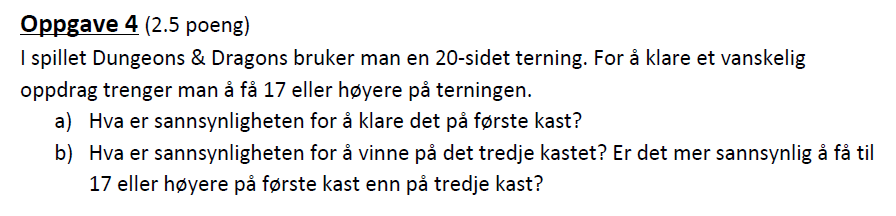
\includegraphics[scale = 0.7]{../figures/oppgave4b.png}
\caption{Oppgave 4}
\label{fig:oppgave4}
\end{figure}
I oppgave b står det \emph{Hva er sannsynligheten for å vinne på det tredje kastet?}. Her var hensikten at
elevene skulle oppfatte det som \emph{Hva er sannsynligheten for å tape på to runder på rad og deretter vinne på 
det tredje kastet?}, men mange oppfattet det som å vinne på tredje kastet uavhengig av hva som forekommer på de 
første to kast. Dermed ville svaret til neste del av deloppgaven, \emph{Er det mer sannsynlig å få til 17 eller 
høyere på første kast enn på det tredje kast?},  være ``like sannsynlig'' og det var ofte det elevene besvarte. 
I oppgave 4.b har elevene anledning til å demonstrere høyt kompetansenivå. Dessverre er formuleringen ikke
godt nok til å trekke elevene inn i et diskurs. Her burde det gjerne ha blitt lagt til en bisetning, som 
for eksempel \emph{``Kan du gi en forklaring?''}. Med slike spørsmål er det lettere å oppdage elevenes
feiltolkninger, fordi da slipper en å få besvarelser som er enten ``ja'' eller ``nei''. Oppgave 
5.b var bedre formulert (se vedlegg 1). Her kreves det eksplisitt en forklaring fra elevene.
Dette er en fin øvelse for elever å demonstrere at de har forstått bruken av utfallstreet. Det var derimot
få elever som fikk til oppgaven, og enda fære som prøvde å gi en forklaring. Etter å snakket med elevene
som forsøkte å løse oppgaven, var forklaringen deres at enten så overså de krav om begrunnelsen, eller de var
ikke sikker på forklaringen. De som overså krav om begrunnelsen, neglisjerte denne delen av oppgaven fordi
de fikk ikke med seg at det skulle legges til en forklaring, og de andre svarte at en forklaring var ikke
viktig å få med. 

\begin{figure}
\centering
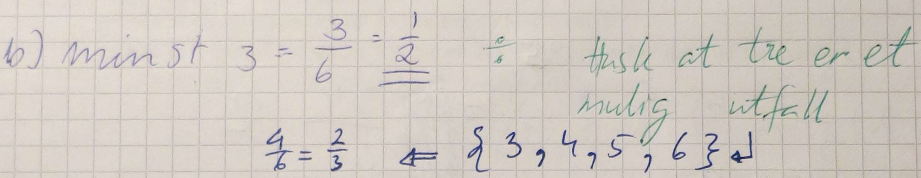
\includegraphics[scale = 0.4]{../figures/maryam.png}
\caption{Oppgave 1}
\label{fig:maryam}
\end{figure}

\begin{figure}
\centering
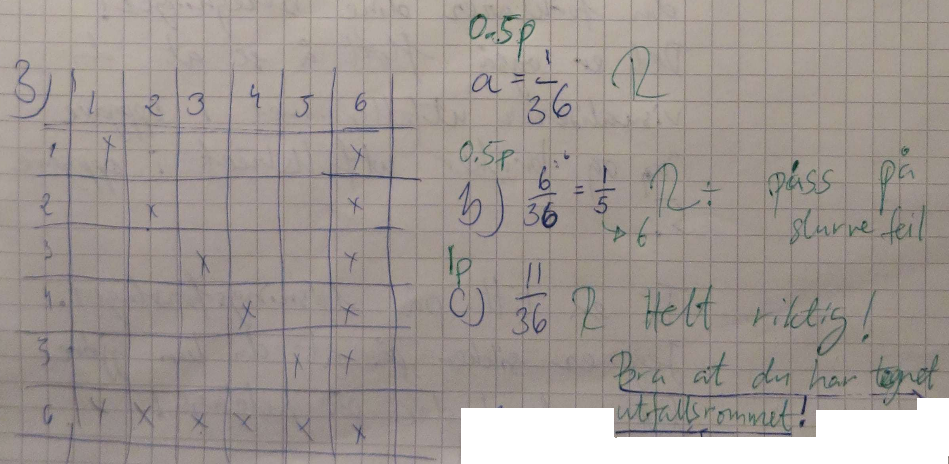
\includegraphics[scale = 0.4]{../figures/maryam2.png}
\caption{Oppgave 3}
\label{fig:maryam2}
\end{figure}

\begin{figure}
\centering
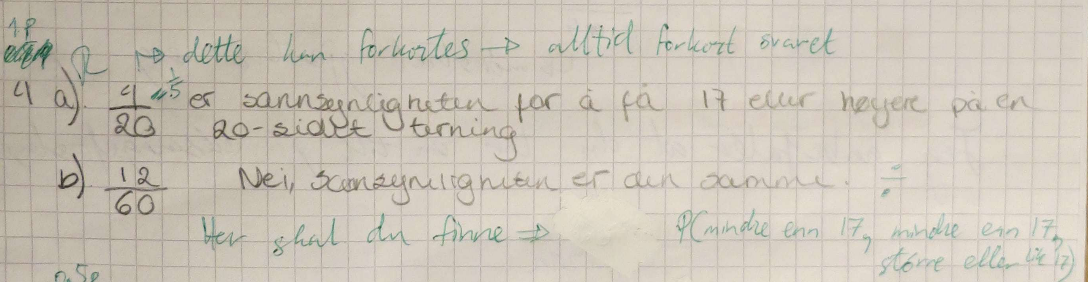
\includegraphics[scale = 0.4]{../figures/maria.png}
\caption{Oppgave 4}
\label{fig:maria}
\end{figure}

\begin{figure}
\centering
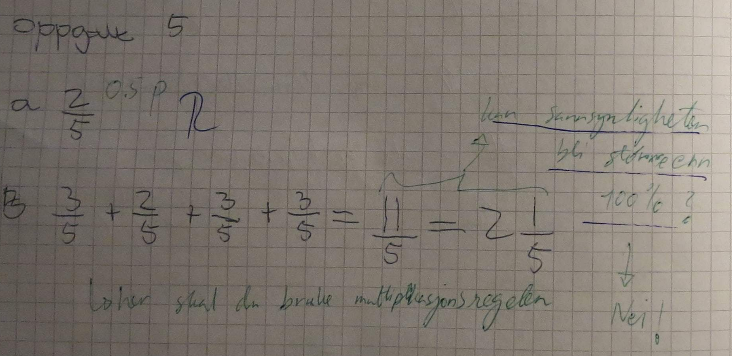
\includegraphics[scale = 0.4]{../figures/mohsin.png}
\caption{Oppgave 5}
\label{fig:mohsin}
\end{figure}


\subsection*{Tilbakemeldinger}

William redegjør for hvorfor tilbakemeldinger noen ganger kan føre til senking 
i elvenes ytelse. Han referer til Kluger og DeNisi (1996), når han summerer opp 
\begin{displayquote}
\textelp{} feedback was least effective when it focused on the task in hand, 
and more effective when it focused on the details at hand, and most effective 
when it focused on the details of the task and involved goal-setting.
(\citeNP[s. 140]{will10})
\end{displayquote}

\begin{figure}
\centering
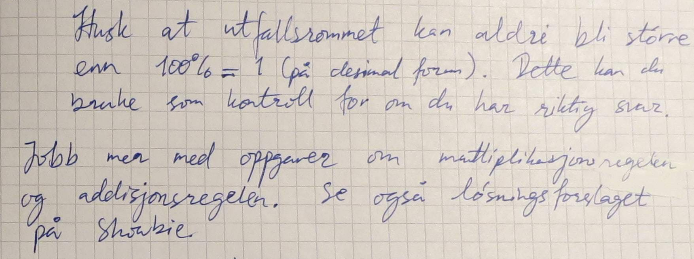
\includegraphics[scale = 0.4]{../figures/mohsin2.png}
\caption{Tilbakemelding og fremovermelding}
\label{fig:mohsin2}
\end{figure}

Et problem som jeg opplevde med kartleggingsprøven var at elever demonstrerte ikke like sterk engasjement
i å besvare riktig. Jeg snakket med en av de sterke elevene som jeg har tidligere observert i timene.
Jeg spurte hen hvorfor hen ikke hadde besvart en spesifikk oppgave og hen svarte med å si at oppgaven 
var lett, men hen ``orket'' ikke å gå gjennom den. Grunnen hen oppga var at siden det ikke var en prøve,
hadde det ikke så mye betyning. Dette samsvarer godt med det \citeA[s. 3]{brbl14} skriver : \emph{Vurdering 
kan ha en betydelig påvirkning på hvordan elever jobber, fordi de oppfatter det som vurderes som det eneste
``som teller''}.


\end{document}
